\chapter{Amateur Radio Direction Finder Receiver}

The circuit is designed in KiCad - \cite{kicad}

\begin{enumerate}
\item
The radio receiver:\\
	The main blocks:
	\begin{itemize}
	\item 9 turns from 210 cm CuZ copper wire as antenna,
	\item RF (radiofrequency) amplifier,
	\item RF band pass filter,
	\item BJT (bipolar junction transistor) based mixer,
	\item local oscillator,
	\item audio frequency low pass filter,
	\item audio amplifier.
	\end{itemize}
\item
The test transmitter:\\
	Collpitts type oscillator, where the quartz frequency is some 100 Hz different from the receiver local oscillator frequency, in order to make audio signal and it can be heard.
\end{enumerate}

\newpage
\section{Schematic}

The schematic diagram of the receiver is in Fig. \ref{fig:rokasch}.

\begin{figure}[H]
\centering
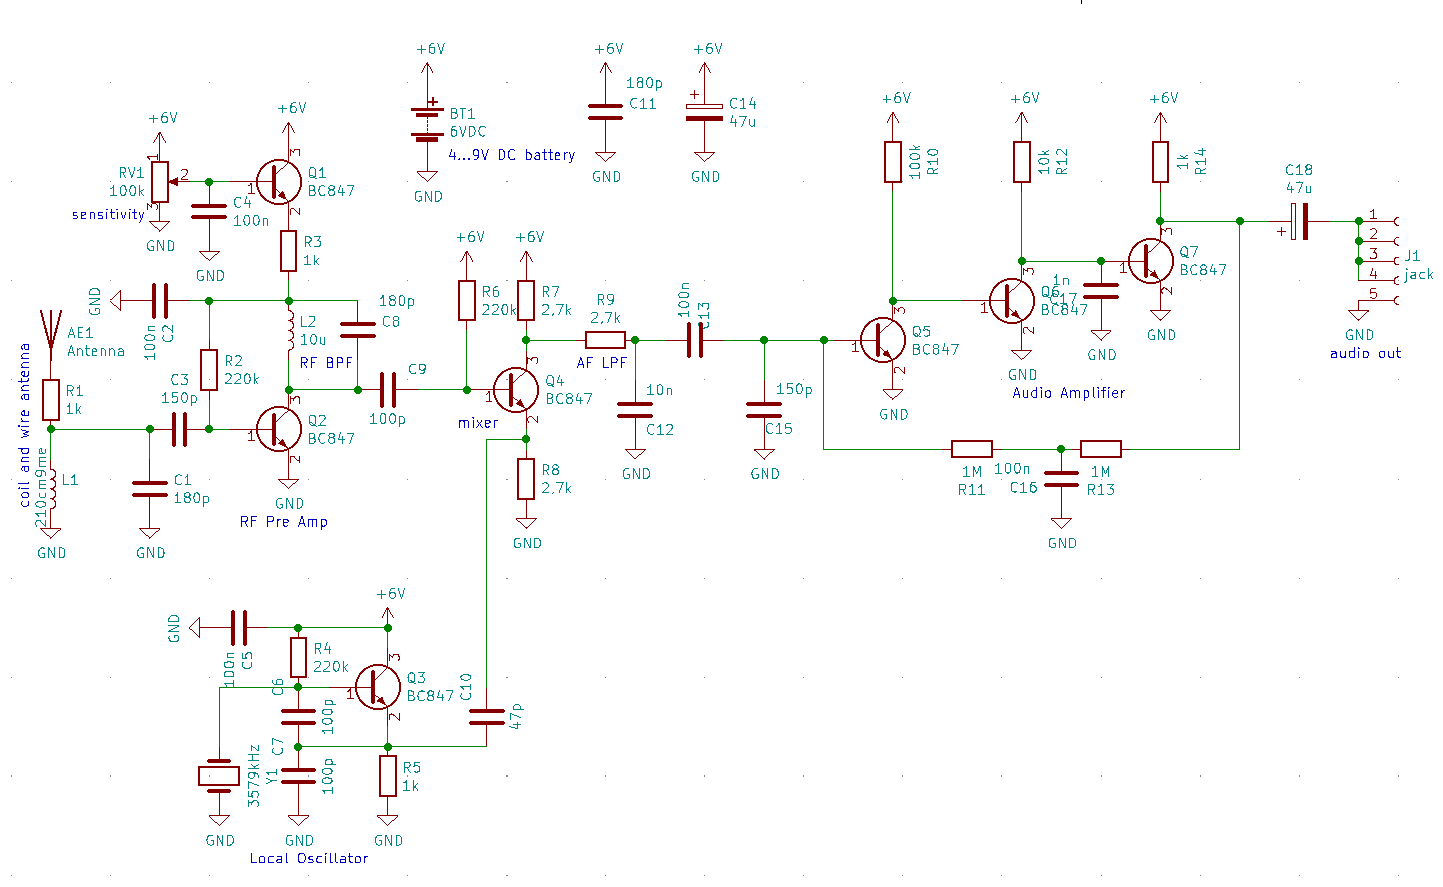
\includegraphics[width=1\textwidth]{../pic/sch.png}\\
\caption{Schematic}
\label{fig:rokasch}
\end{figure}

\newpage
\section{Printed Circuit Board}

The designed PCB can be seen in Fig. \ref{fig:rokanyhl}. There are THT and SMD type components.

\begin{figure}[H]
\centering
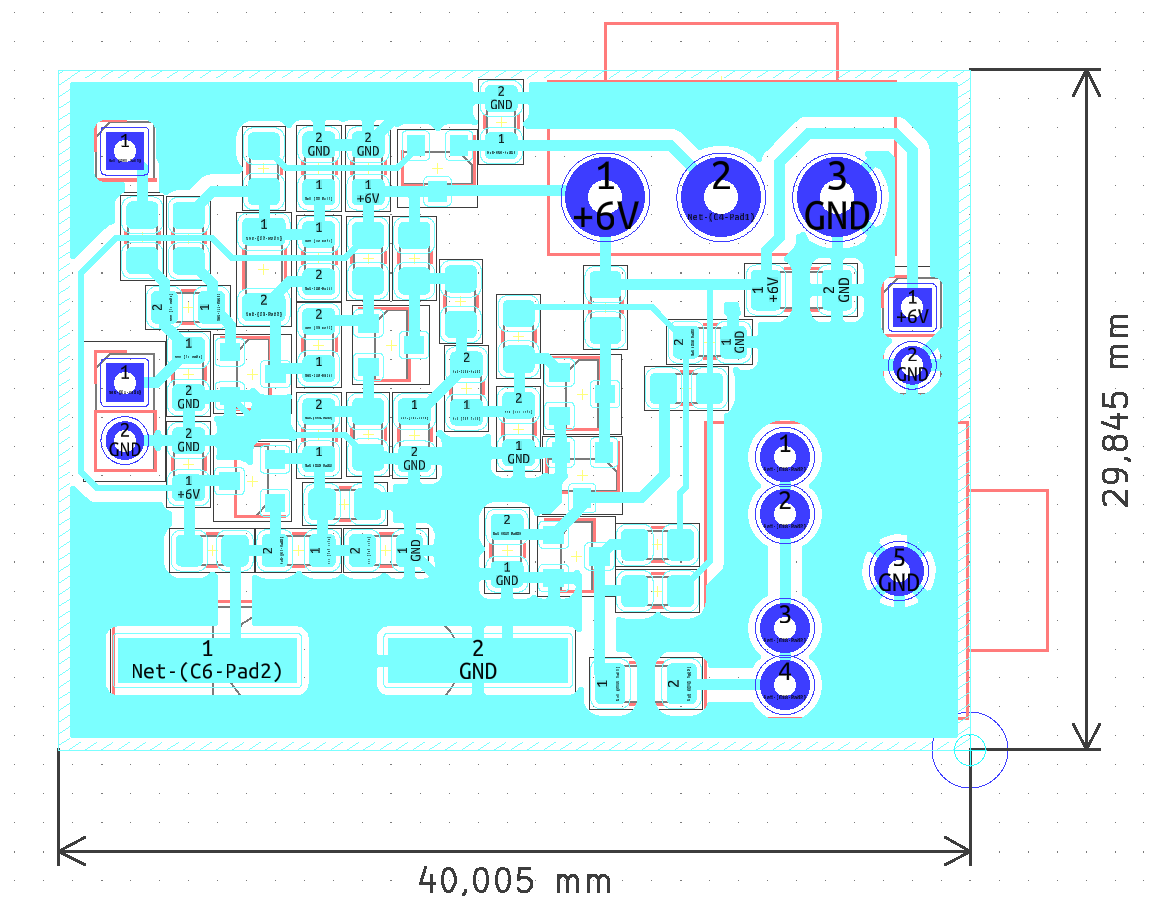
\includegraphics[width=1\textwidth]{../pic/pcb.png}
\caption{PCB}
\label{fig:rokanyhl}
\end{figure}

\newpage
\section{Component placement}

The components with its reference is in Fig. \ref{fig:rokault}.

\begin{figure}[H]
\centering
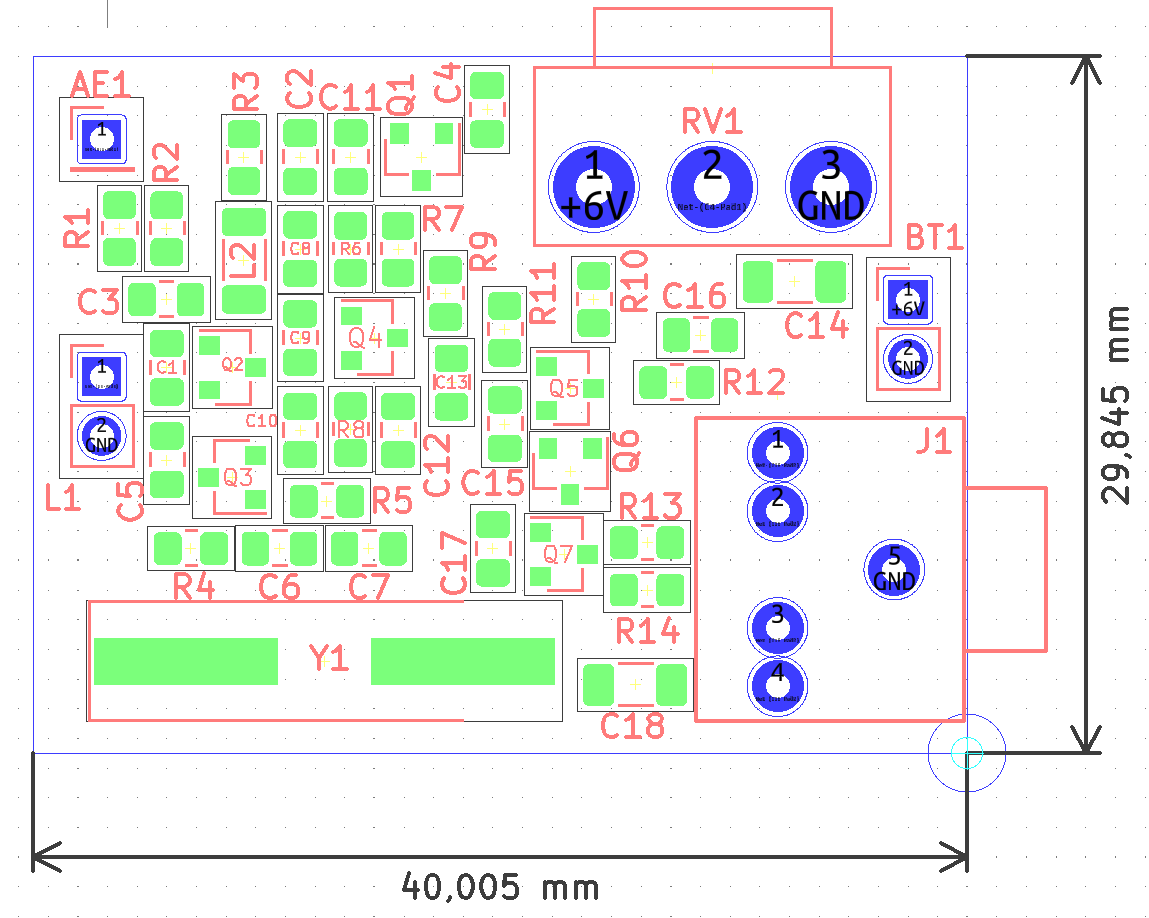
\includegraphics[width=1\textwidth]{../pic/pos.png}
\caption{Components Placement}
\label{fig:rokault}
\end{figure}

Placement order:

\begin{enumerate}
\item resistors,
\item capacitors,
\item inductors,
\item transistors,
\item connectors,
\item antenna.
\end{enumerate}

\newpage
\section{Measurement of the realized circuit}

The task is to measure the following parameters of the realized circuit and make test and measurement report based on the measurement results.

\begin{enumerate}
\item Bias DC voltages to the reference GND point on all pins of all semiconductors.
\item Voltage curve in time of the local oscillator output (emitter): peak-to-peak voltage, frequency, png from the scope.
\item Receiver audio (time domain) output signal on the AF output connector: variable resistor low, middle, high position: peak-to-peak voltage, frequency, curve. During this measurement, a single test transmitter will be run near to the receiver.
\end{enumerate}